
\chapter{\IfLanguageName{dutch}{Proof of Concept}{Abstract}}
\label{ch:poc}

In dit hoofdstuk worden de opstellingen met omgevingen voor Hashicorp Vault en Azure Key Vault opgezet. Alle vermelde scripts / playbooks zijn aanwezig op volgende \href{https://github.com/Rayenasr/Secrets-management-thesis}{github repository}\footnote{\href{https://github.com/Rayenasr/Secrets-management-thesis}{github repository}}.

\section{Opzet Hashicorp Vault}

De applicatie wordt opgezet in een virtuele test omgeving, on-premise van het Wolters Kluwer development infrastructuur. Een aantal zaken die aanwezig waren alvorens het begin van de proof of concept (PoC).

\begin{itemize}
    \item Dell laptop binnen het Wolters Kluwer domein met WSL² Ubuntu + ansible 2.10.6  
    \item Virtuele test omgeving binnen Wolters Kluwer domein
    \item API test call script met dank aan de co-promotor
    \item Administrator rechten bij CI/CD tool TeamCity in productie en development
\end{itemize}
\textit{Windows Subsystem for Linux} is een compatibiliteitslaag voor het native draaien van binaire linuxbestanden in een console omgeving op een Windows 10 machine \autocite{wsl2021}. Deze wordt gebruikt om Ansible te laten draaien. Verder zijn de specificaties van de virtuele test omgeving als volgt:

\begin{itemize}
    \item OS: Windows Server 2019 Datacenter (64 bit)
    \item Intel Xeon Silver 4208 CPU @ 2.10GHz
    \item 32GB geheugen
\end{itemize}

\subsection{Installatie \& configuratie Hashicorp Vault}

In onderdeel \ref{ch:ansible}, werd getoond wat Ansible is en hoe deze tool gebruikt wordt om taken te automatiseren. Doorgaans deze PoC zal ansible gebruikt worden voor een aantal taken snel en efficiënt te voltooien. De syntaxis die gebruikt wordt om een Ansible script op te roepen in de WSL² Ubuntu omgeving is als volgt: \textit{ansible-playbook PLAYBOOK.YML -i INVENTORY}. Bij het klaarzetten van de omgeving wordt Ansible gebruikt aan de hand van playbook \href{https://github.com/Rayenasr/Secrets-management-thesis/blob/main/vault/installVault.yml}{\textit{installVault.yml}}\footnote{\href{https://github.com/Rayenasr/Secrets-management-thesis/blob/main/vault/installVault.yml}{installVault.yml op github}} met bijbehorende \href{https://github.com/Rayenasr/Secrets-management-thesis/blob/main/vault/inventory}{inventory file}\footnote{\href{https://github.com/Rayenasr/Secrets-management-thesis/blob/main/vault/inventory}{inventory file op github}}.


\subsubsection{Installatie}
Alvorens het starten, vraagt het playbook om de gebruikersnaam op te geven met bijbehorend wachtwoord. Dit is zo bij elk playbook gedaan zodat we deze gegevens niet rechtstreeks in de inventory file zetten zoals er afgebeeld werd op figuur \ref{fig:inventorypass}. Eens het playbook afgerond is, kan vault opgestart worden via een elevated command prompt. Dit is een command prompt met administrator rechten. De working directory moet dezelfde zijn als de locatie waar \textit{vault.exe} staat. Eens in deze locatie wordt de commando \textit{vault server -config=.\symbol{92}config\symbol{92}config.hcl} gebruikt om vault op te starten met bijbehorende configuratie bestand. 

\begin{figure}[hbtp]
    \caption{inhoud initieel configuratie bestand}
    %\label{code.1}
    \begin{lstlisting}[language=yaml,frame=single]
1.    ui = true
2.    disable_mlock = true
3.    storage "file" {
4.    path = "./data"
5.    }
6.    listener "tcp" {
7.    address     = "0.0.0.0:8200"
8.    tls_disable = "true"
9.    }
10.   api_addr = "http://127.0.0.1:8200"
11.   #cluster_addr = "https://127.0.0.1:8201"
    \end{lstlisting}
\end{figure}
Vault kan worden opgestart in \textit{dev} modus waar de lokale CLI geauthenticeerd is om met vault te communiceren. basis configuraties zijn in deze modus verwerkt en dient als testomgeving. Data wordt (geëncrypteerd) in vluchtige geheugen opgeslagen. Bij het afsluiten van de vault applicatie is alle toegevoegde data verloren. Omdat we bij deze PoC data willen opslaan en de vault omgeving geregeld afgesloten moet worden, is hier gekozen voor een simpel bestandssysteem. In het configuratiebestand wordt dit vermeld. Vault zal de backend bestanden lokaal creëren en encrypteren. Elke keer wanneer men de vault wilt opstarten zal deze in een sealed state zijn. Wanneer vault sealed is verwacht hij de master key om encryptie uit te voeren. Wanneer men de webpagina \textbf{http://127.0.0.1:8200} voor de eerste keer bezoekt, wordt een pagina weergeven om de master key op te delen in een aantal key shares. Verder wordt er ook opgegeven hoeveel key shares er nodig zijn om vault te openen. Deze key shares vormen het vermogen om de master key terug op te bouwen. Bij deze PoC kiezen we voor vijf key shares met drie nodige keys om de master key terug op te bouwen en de vault te openen. Vervolgens kan men een JSON bestand downloaden waar de vijf key shares in staan met een root token. Dit bestand moet zeer goed worden bewaard. Deze key shares zijn nodig om vault te openen wanneer deze sealed is. Indien deze key shares verloren gaan kan men vault op geen andere manier meer openen en is de data verloren! De bijbehorende root token wordt gebruikt om als root gebruiker te authenticeren. Dit is in het begin nodig om policies en gebruikers aan te maken. Verder moet het gebruik van de root key in een productieomgeving tot een minimum gehouden worden.

\begin{figure}[htbp]
\centerline{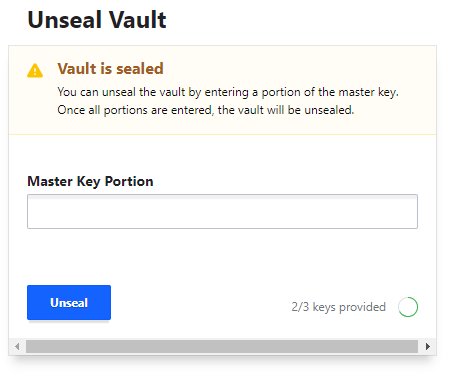
\includegraphics[width=300]{bachproef/img/poc/unsealVault.png}}
\caption{proces om sealed vault te openen \autocite{vault}}
\end{figure}

\subsubsection{Configuratie}
\label{ch:config}

De root key wordt gebruikt om men aan te melden als root gebruiker. Nu men aangemeld is op vault kan men operaties verrichten binnen dit systeem. Hier worden in de volgende delen configuraties verricht:
\begin{itemize}
    \item Secrets (Secrets Engines)
    \item Policies (ACL Policies)
    \item Access (Authentication Methods)
\end{itemize}

Allereerst wordt een nieuwe \textit{secrets engine} aangemaakt. Een secrets engine is een component die data opslaat, encrypteert of decrypteert. Hier wordt er gekozen voor een kv secrets engine aan te maken. Alle standaard waarden worden behouden. Eens deze engine aangemaakt is, kan men hier secrets opslaan met een key-value methode. Hier maken we een secret aan waar we later key-value gegevens aan toe voegen. Deze geven we de naam \textit{TeamCity}. Hierin worden twee secrets aangemaakt, namelijk de keys \textit{TeamCityAccount} en \textit{TeamCityAccountEncryptedPassword} met bijbehorende waarden.
\newline

Vervolgens worden de policies aangemaakt. Hier worden 2 policies aangemaakt, namelijk \textit{teamcity} en \textit{admin}. Dit wordt verricht door een ACL policy aan te maken. Om dit te doen kunnen we via de web ui een policy definiëren. Deze kan ook worden opgeladen. Via ansible laten we het playbook \href{https://github.com/Rayenasr/Secrets-management-thesis/blob/main/vault/createPolicyFiles.yml}{createPolicyFiles.yml}\footnote{\href{https://github.com/Rayenasr/Secrets-management-thesis/blob/main/vault/createPolicyFiles.yml}{createPolicyFiles.yml op github}} lopen om twee HCL bestanden aan te maken waar de policies voor de beide rollen in gedefinieerd staan. Deze worden in de plugin directory gestoken. Voor admin wordt de naam \textit{admin} opgegeven en bijbehorende HCL bestand wordt hierbij opgeladen. Ditzelfde gebeurt ook voor de teamcity policy met naam \textit{teamcity}.

\begin{figure}[htbp]
\centerline{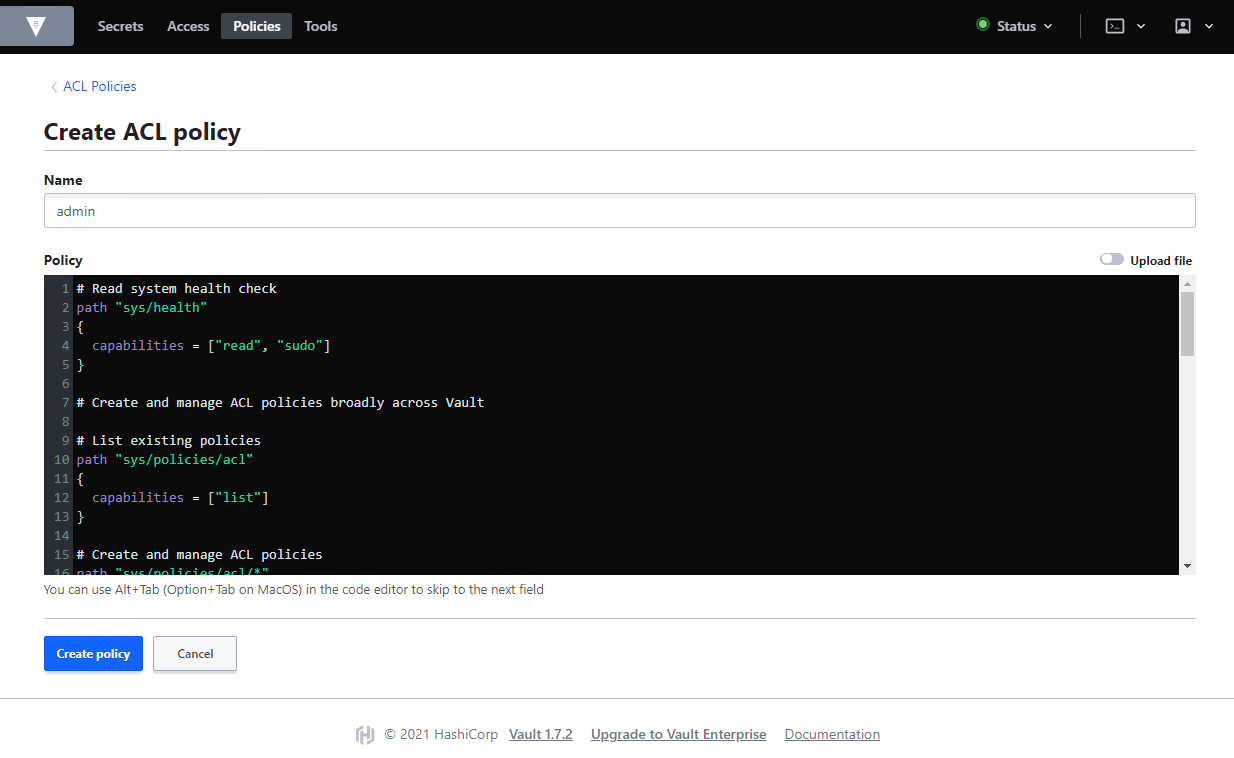
\includegraphics[width=400]{bachproef/img/poc/acl policy.png}}
\caption{proces voor policy aan te maken \autocite{vault}}
\end{figure}

Nu wordt er gekeken naar de access tab. Hier kan men methodes toevoegen om authenticatie te verrichten. Men kan een \textit{userPass} authenticatie methode toevoegen om met gedefinieerde gebruikersnamen met bijbehorende wachtwoorden, aan te melden op het systeem. Dit zal hier niet worden gedaan omdat in deel \ref{ch:ldap} een integratie wordt uitgevoerd met LDAP om AD gegevens te gebruiken binnen het domein van Wolters Kluwer. Er wordt nu wel al een \textit{Approle} toegevoegd. Deze dient als authenticatie methode voor applicaties onder een bepaalde rol. Deze rol wordt aangemaakt zodat via de TeamCity integratie, later secrets kunnen worden opgehaald vanuit vault. De configuratie hiervoor wordt via de CLI van de vault UI uitgevoerd. De configuratie wordt weergeven met output waarden in figuur \ref{ch:role}. Van deze waarden worden later de role\_id en secret\_id values gebruikt voor de plugin integratie met TeamCity.
\newpage


\begin{figure}[htbp]
\centerline{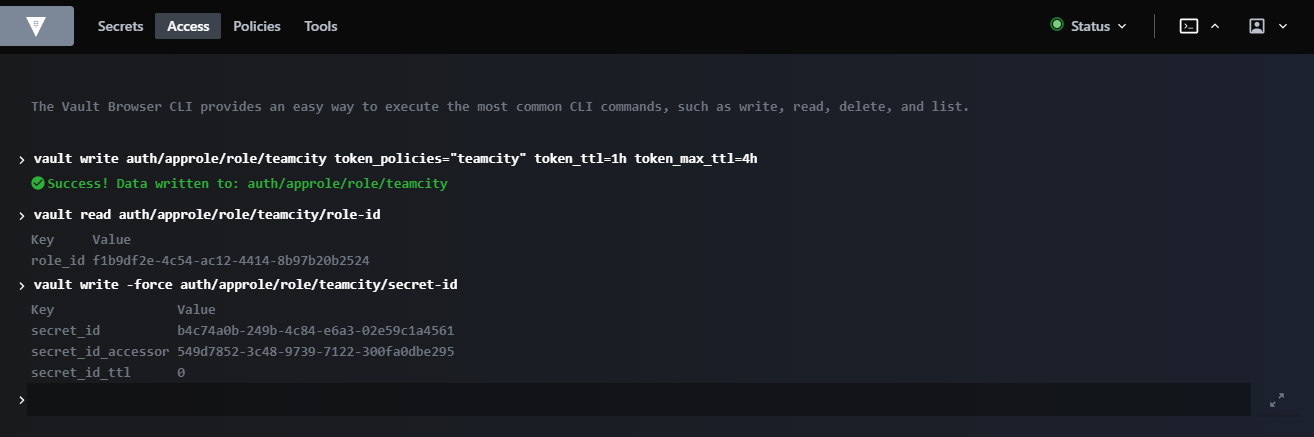
\includegraphics[width=500]{bachproef/img/poc/approle aanmaken.png}}
\caption{proces voor approle aan te maken \autocite{vault}}
\label{ch:role}
\end{figure}

\subsection{LDAP integratie}
\label{ch:ldap}

In een vorig onderdeel werd er gesproken over de access tab waar authenticatie methodes worden toegevoegd. Nu wordt vault geïntegreerd met LDAP zodat gebruikers van het development team zich kunnen verbinden met vault als een gebruiker. Er wordt gekozen voor een nieuwe authenticatie methode. Hier wordt LDAP gekozen. De standaard waarden worden behouden en de methode wordt geactiveerd. Vervolgens komt de configuratie om vault met LDAP te verbinden. Hier wordt de URL gegeven van de domeincontroller: \textit{ldap://EXAMPLE.local:389}. Vervolgens wordt bij User Attribute de waarde \textit{samaccountname} gegeven. Zo kunnen gebruikers via hun gebruikersnaam aanmelden die ze gewoon zijn, bijvoorbeeld \textit{John.Doe}. Vervolgens wordt het bindDn gegeven waarmee gebruikers opgezocht worden \textit{CN=EXAMPLE-IT-LDAP,OU=Service Accounts,OU=EXAMPLE,DC=DC-EXAMPLE} en de userDn \textit{DC=DC-EXAMPLE} met bijbehorende bindpass. Eens dit gelukt is kunnen gebruikers van Wolters Kluwer een verbinding maken met vault. Nu moet er een groep worden aangemaakt waar gebruikers aan toegevoegd worden voor admin rechten. Binnen de LDAP authenticatie methode, maakt men een groep aan genaamd \textit{poc users} met de \textit{admin} policy. Vervolgens kunnen gebruikers worden toegevoegd zodat deze de policy verkrijgen.

\begin{figure}[htbp]
\centerline{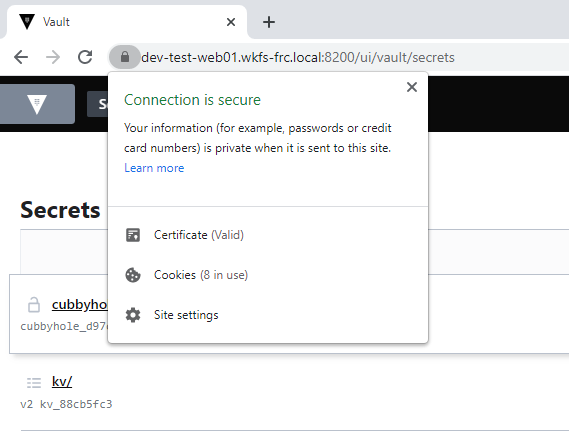
\includegraphics[width=300]{bachproef/img/poc/secure.png}}
\caption{Beveiligde webapplicatie \autocite{vault}}
\label{fig:secure}
\end{figure}
\newpage

\subsection{Installatie SSL certificaat}
In dit onderdeel wordt een SSL certificaat aangemaakt en toegevoegd aan de PoC. Dit is nodig voor het verkeer te beveiligen tussen clients en de vault webpagina. Binnen Wolters Kluwer is dit een requirement om aan te voldoen bij webapplicaties. Om dit te behalen wordt de applicatie \href{https://www.digicert.com/}{\textit{Digicert}\footnote{\href{https://www.digicert.com/}{Digicert website}}} gebruikt. Hiermee wordt een certificaat aanvraag opgesteld die verder behandelt wordt door \textit{Microsoft Active Directory Certificate Services}. Hier wordt de aanvraag verwerkt en verkrijgt men een \textit{certnew.p7b} bestand. Hier is het certificaat in opgeborgen. Daarna gaat men terug naar de Digicert applicatie en wordt dit bestand geïmporteerd. Hieruit kan men vervolgens drie bestanden downloaden. Een \textit{CAcert.crt} bestand en twee andere bestanden behorende tot de host waarvoor de certificaten getekend zijn. In dit geval is dat \textit{dev-test-web01\_wkfs\_local.crt} en \textit{dev-test-web01\_wkfs-frc\_local.key}. Deze drie bestanden worden in de map \textit{certs} gestoken onder \textit{config}. In het configuratie bestand moet er worden verwezen naar deze certificaten. TLS moet ook worden geactiveerd. Het adres \textbf{http://127.0.0.1:8200} zou ook niet meer gebruikt worden, het FQDN \textbf{https://dev-test-web01.wkfs-frc.local:8200} zal hier gebruikt worden. Vervolgens moet de omgevingsvariabele in het systeem ook verandert worden zodat deze ook het juiste adres zal gebruiken. Dit wordt allemaal behaald via het playbook \href{https://github.com/Rayenasr/Secrets-management-thesis/blob/main/vault/updateConfigFile.yml}{updateConfigFile.yml}\footnote{\href{https://github.com/Rayenasr/Secrets-management-thesis/blob/main/vault/updateConfigFile.yml}{updateConfigFile.yml op github}}. Eens het configuratie bestand is bijgewerkt wordt vault opnieuw opgestart om deze te gebruiken. In figuur \ref{fig:ssl} kan men het proces bekijken hoe het resultaat van \ref{fig:secure} behaald werd. 


\begin{figure}
    \centering
    \subfigure[]{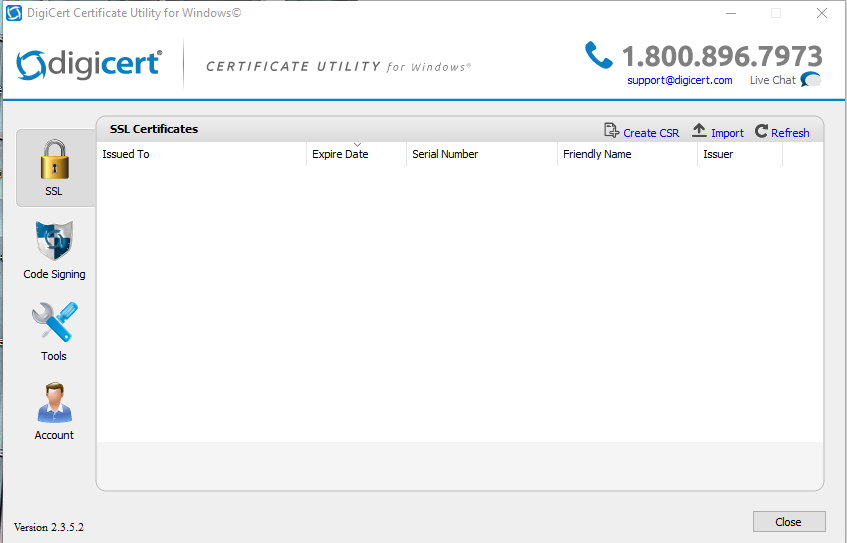
\includegraphics[width=0.4\textwidth]{bachproef/img/poc/digicert.png}}
    \subfigure[]{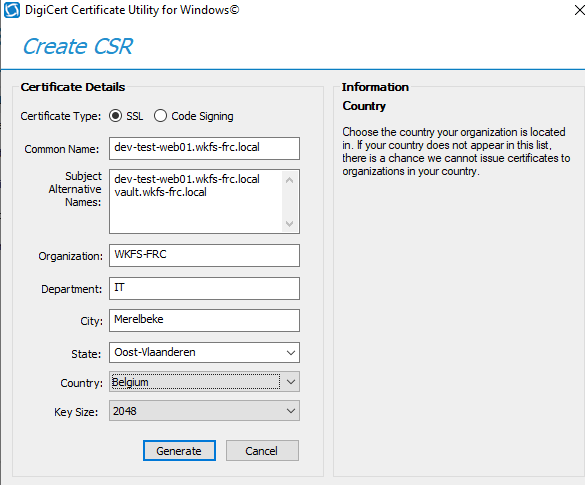
\includegraphics[width=0.4\textwidth]{bachproef/img/poc/1ssl.png}} 
    \subfigure[]{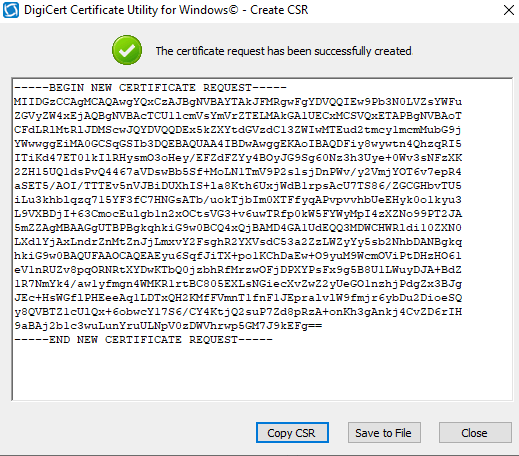
\includegraphics[width=0.4\textwidth]{bachproef/img/poc/2ssl.png}} 
    \subfigure[]{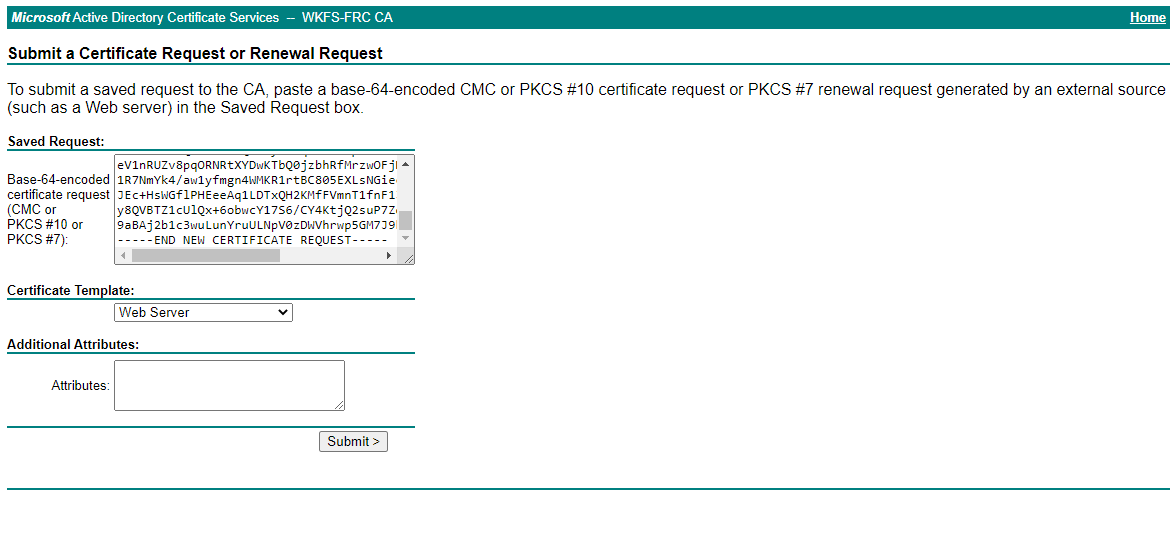
\includegraphics[width=0.4\textwidth]{bachproef/img/poc/3ssl.png}}
    \subfigure[]{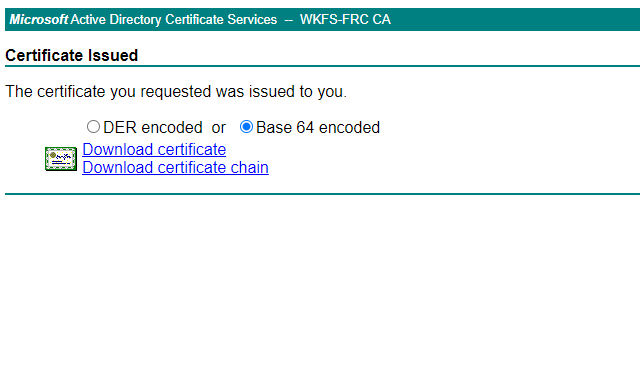
\includegraphics[width=0.4\textwidth]{bachproef/img/poc/4ssl.png}}
    \subfigure[]{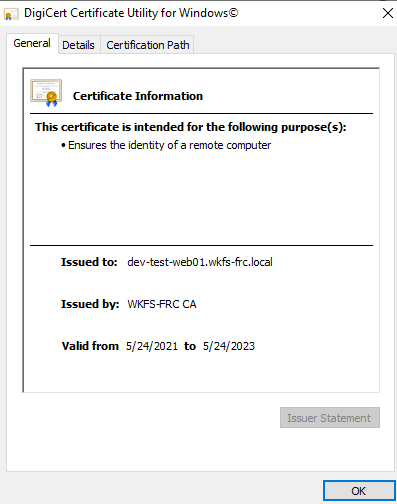
\includegraphics[width=0.4\textwidth]{bachproef/img/poc/5ssl.png}}
    \caption{proces om SSL certificaat te tekenen \autocite{digicert}}
    \label{fig:ssl}
\end{figure}

\newpage
\section{Opzet Azure Key Vault}
\label{ch:azurekey}

Het opzetten van een Key Vault van Azure is minder complex dan een on-premise secrets management opstelling zoals bij Hashicorp Vault. Toch zijn er enkele stappen die uitgevoerd moeten worden voor secrets beheerd kunnen worden. Als eerste wordt een nieuwe resource group aangemaakt. Deze krijgt de naam \textit{rg-devsup-keyvault}. Hier maken we een nieuwe resource. We kiezen voor key vault en noemen deze \textit{kv-devsup}. De recent aangemaakte resource group wordt hier gekozen en de resterende opties worden niet gewijzigd. Hiermee bekomen we tot het resultaat afgebeeld in figuur \ref{fig:azure}.

Vervolgens wordt een \textit{service principal} aangemaakt voor de key vault die gebruikt zal worden door de integratie plugin van Azure Key Vault en TeamCity. Dit wordt behaald via de Azure CLI met commando \textit{az ad sp create-for-rbac --name TeamCityVault}. Vervolgens moeten we enkele waarden verkrijgen over deze service principal die later nodig zijn bij de integratie. Via volgende commando's wordt dit behaald: \textit{az account show --query '{tenantId:tenantId,subscriptionid:id}';} en \textit{az ad sp list --display-name TeamCityVault --query '{clientId:[0].appId}'}. Deze commando's werden door een persoon verricht met bevoegdheden aan Azure AD binnen het Wolters Kluwer domein. De aangemaakte service principal wordt juist nog toegevoegd bij de gebruikers van de key vault. Dit gebeurt via de access policies tab binnen de \textit{kv-devsup} key vault. Dit staat ook afgebeeld op figuur \ref{fig:azure}. Hier wordt de service principal \textit{TeamCityVault} gekozen en toegevoegd met de \textbf{GET} key permission. De service principal moet juist de rechten hebben om secrets op te halen. Nu worden twee secrets aangemaakt in deze vault. Net zoals bij Hashicorp Vault, worden de keys \textit{TeamCityAccount} en \textit{TeamCityAccountEncryptedPassword} met bijbehorende waarden toegevoegd.
\begin{figure}[htbp]
\centerline{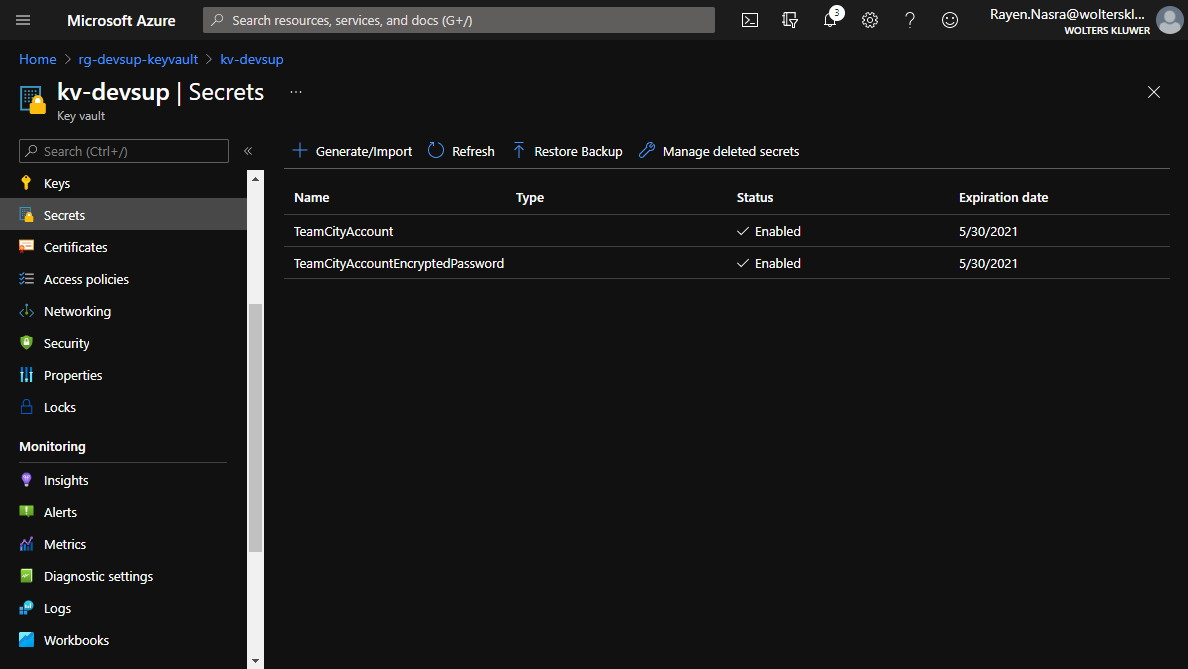
\includegraphics[width=400]{bachproef/img/poc/azurekeyvault.png}}
\caption{Aangemaakte Key Vault in Azure \autocite{azure}}
\label{fig:azure}
\end{figure}

\section{TeamCity omgeving}
\subsection{Integratie tools met TeamCity}

In dit gedeelte worden de integratie plugins geïnstalleerd op TeamCity. Hierna worden connecties vastgelegd met de Azure Key Vault en Hashicorp Vault. Als eerste wordt het playbook \href{https://github.com/Rayenasr/Secrets-management-thesis/blob/main/vault/fetchPlugins.yml}{\textit{fetchPlugins.yml}}\footnote{\href{https://github.com/Rayenasr/Secrets-management-thesis/blob/main/vault/fetchPlugins.yml}{fetchPlugins.yml op github}} gebruikt om de beide plugins te downloaden en klaar te zetten in de vault directory onder \textit{plugins}. Hierna worden deze op de webapplicatie van TeamCity opgeladen via volgende stappen:

\begin{enumerate}
  \item Op het homescreen van TeamCity kiest men voor het tandwiel icoon (Administration)
  \item Nu kiest men voor \textit{plugins} onder \textit{Server Administration}
  \item Hier laad men elke plugin afzonderlijk op
  \item De toegevoegde plugins worden ingeladen en zijn klaar voor gebruik
\end{enumerate}

Er is een project aangemaakt dat dient als test case. Om hier de Azure Key Vault plugin en de Hashicorp Plugin te gebruiken moeten eerst connecties worden vastgelegd. Hier worden de eerder aangemaakte approle van vault, en de service principal van azure voor gebruikt. Dit wordt behaald via volgende stappen:

\begin{enumerate}
  \item Het Secret Management project word gekozen onder \textit{Development Support\symbol{92}Playground\symbol{92}Secret Management}
  \item Hier kiest men voor \textit{edit project settings}
  \item Verder wordt onder \textit{General Settings}, \textit{Connections} gekozen
  \item Hier worden voor zowel Hashicorp Vault als Azure Key Vault een connectie toegevoegd. Voorbeeld bij figuur \ref{fig:connections}
\end{enumerate}

\begin{figure}[!htb]
    \centering
    \subfigure[Azure Key Vault]{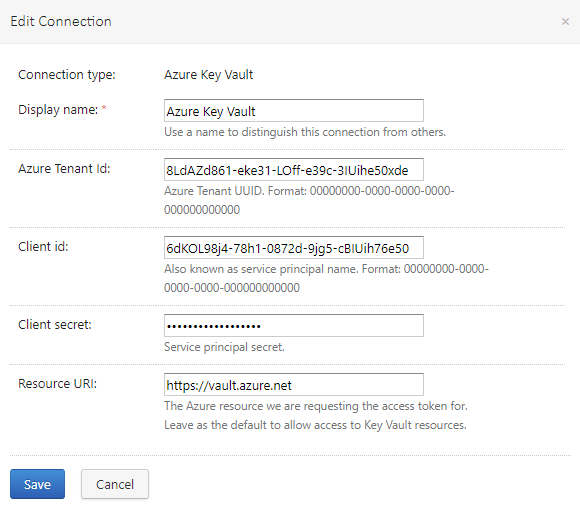
\includegraphics[width=0.4\textwidth]{bachproef/img/poc/KeyVaultConnection.png}}
    \subfigure[Hashicorp Vault]{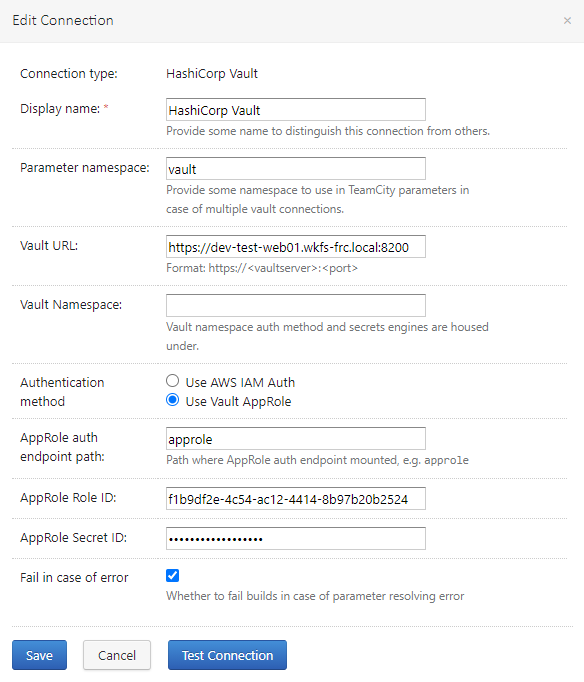
\includegraphics[width=0.4\textwidth]{bachproef/img/poc/VaultConnection.png}} 
    \caption{proces connecties toe te voegen \autocite{teamcity}}
    \label{fig:connections}
\end{figure}

\subsection{Secret Management Project}
In TeamCity is er een project voorzien om meerdere build configuraties aan te maken. Voor Azure Key Vault en Hashicorp Vault worden twee verschillende build configuraties opgesteld onder hetzelfde project. De plugins doen hun werking aan de hand van omgevingsvariabelen die alvorens deployments van builds worden gedeclareerd. De plugins doen hun werking wanneer deze variabelen worden meegegeven als script argumenten. Hierdoor worden deze opgehaald en toegevoegd aan het proces van de build. Dit wordt behaald onder de configuratie opties van het project, onder \textit{parameters}. Omgevingsvariabelen worden gedeclareerd met het prefix `\textit{.env}`. Zo kan een variabele met naam \textit{env.AgentsAmount} worden aangemaakt met een vaste waarde. Voor de Hashicorp Vault plugin geldt volgende syntaxis `\textbf{\%vault:PATH!KEY\%}`. Voor Azure key vault is dat `\textbf{\%keyvault:VAULT NAME/SECRET NAME\%}`. De waarden waar naar gerefereerd moet worden zijn de waarden die in deel \ref{ch:config} reeds toegevoegd zijn geweest bij hashicorp vault. Voor azure key vault werd dit gedaan in deel \ref{ch:azurekey}. Op figuur \ref{fig:envvar} staan voorbeelden waar deze variabelen worden toegevoegd.
%Volgende variabelen worden toegevoegd voor de hashicorp vault build: \textit{env.TeamCityAccount} met waarde\textit{\%vault:kv/TeamCity!/TeamCityAccount\%}, vervolgens variabele  \textit{env.TeamCityAccountEncryptedPassword} met waarde \textit{\%vault:kv/TeamCity!/TeamCityAccountEncryptedPassword2\%} toegevoegd. 

%Het formaat voor de azure key vault variabele is als volgt \textbf{\%keyvault:<vault name>/<secret name>\%}. Hiermee worden in de andere configuratie build volgende omgevingsvariabelen opgegeven: \textit{env.TeamCityAccount} met waarde \textit{\%keyvault:kv-devsup/TeamCityAccount\%}, vervolgens variabele \textit{env.TeamCityAccountEncryptedPassword} met waarde \textit{\%keyvault:kv-devsup/TeamCityAccountEncryptedPassword\%} 

\begin{figure}[!htb]
    \centering
    \subfigure[Azure Key Vault]{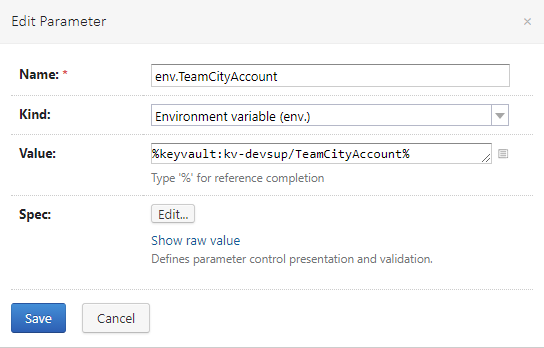
\includegraphics[width=0.45\textwidth]{bachproef/img/poc/AzureParam.png}}
    \subfigure[Hashicorp Vault]{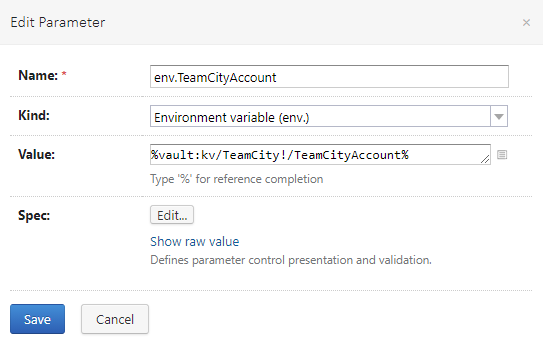
\includegraphics[width=0.45\textwidth]{bachproef/img/poc/VaultParam.png}} 
    \subfigure[Azure Key Vault]{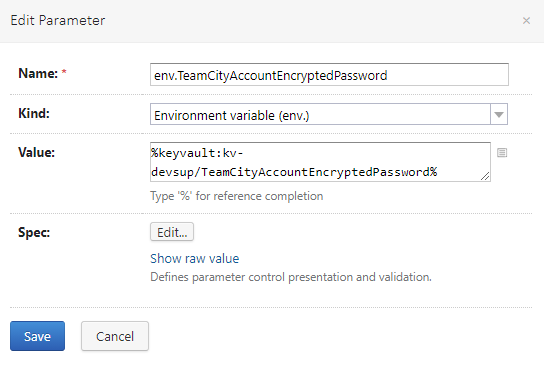
\includegraphics[width=0.45\textwidth]{bachproef/img/poc/AzureParam2.png}}
    \subfigure[Hashicorp Vault]{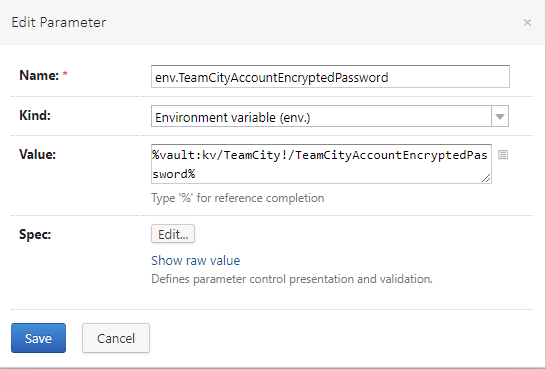
\includegraphics[width=0.45\textwidth]{bachproef/img/poc/VaultParam2.png}} 
    \caption{omgevingsvariabelen toevoegen \autocite{teamcity}}
    \label{fig:envvar}
\end{figure}
\newpage
Voor beide build configuraties worden dezelfde build steps aangemaakt. Hier wordt een powershell script \href{https://github.com/Rayenasr/Secrets-management-thesis/blob/main/TeamCity/RunJobWithVault.ps1}{RunJobWithVault.ps1}\footnote{\href{https://github.com/Rayenasr/Secrets-management-thesis/blob/main/TeamCity/RunJobWithVault.ps1}{RunJobWithVault.ps1 op github}} opgeroepen waar de omgevingsvariabelen meegegeven worden. Deze worden toegevoegd aan het \textit{Scrip argument} gedeelte als ``\textbf{"\%env.TeamCityAccount\%"}`` en ``\textbf{"\%env.TeamCityAccountEncryptedPassword\%"}``. Dit is het gedeelte waar de plugins de syntaxis van de variabelen zullen opmerken eens deze opgeroepen worden bij builds. Deze gegevens kunnen worden opgeslagen en verborgen gehouden in het TeamCity systeem waar ze gemaskeerd worden. Deze worden dus niet geëncrypteerd. In deze instantie worden de waarden geleverd door de vaults van Hashicorp en Azure. Dit voegt een extra abstractielaag tussen TeamCity en gebruikte secrets. Wanneer een build wordt opgeroepen wordt een bepaalde agent die inactief is, verwezen om de uitvoering te doen. Bij deze build wordt het script opgeroepen vanuit een netwerkshare en worden de omgevingsvariabelen meegegeven. Het script zal ervoor zorgen dat een API call naar de TeamCity server wordt gemaakt met gegevens van een administrator, waarmee een andere build wordt gestart. Deze tweede build heeft als enige werking een output te geven met de gebruikte secrets van de vorige build. Met andere woorden worden in beide scripts de secrets opgeroepen. In het tweede script wilt hij deze dan effectief in de output weergeven.

De werking van de Azure Key Vault build wordt in figuur \ref{fig:azurescripts} afgebeeld. Hier kan men opmerken dat de secrets via de eerder ingestelde connectie worden opgehaald. In de build agent wordt de access token in het vluchtige geheugen opgenomen waarmee toegang wordt aangevraagd aan Azure AD, gelimiteerd tot de key vault \textit{kv-devsup}. De secrets worden geleverd als een wachtwoord parameter. De TeamCity server heeft nooit toegang tot de secrets en deze operaties worden meten gedelegeerd aan de build agent. \autocite{azurekvplug}

\begin{figure}[!htb]
    \centering
    \subfigure[API Call met secrets request]{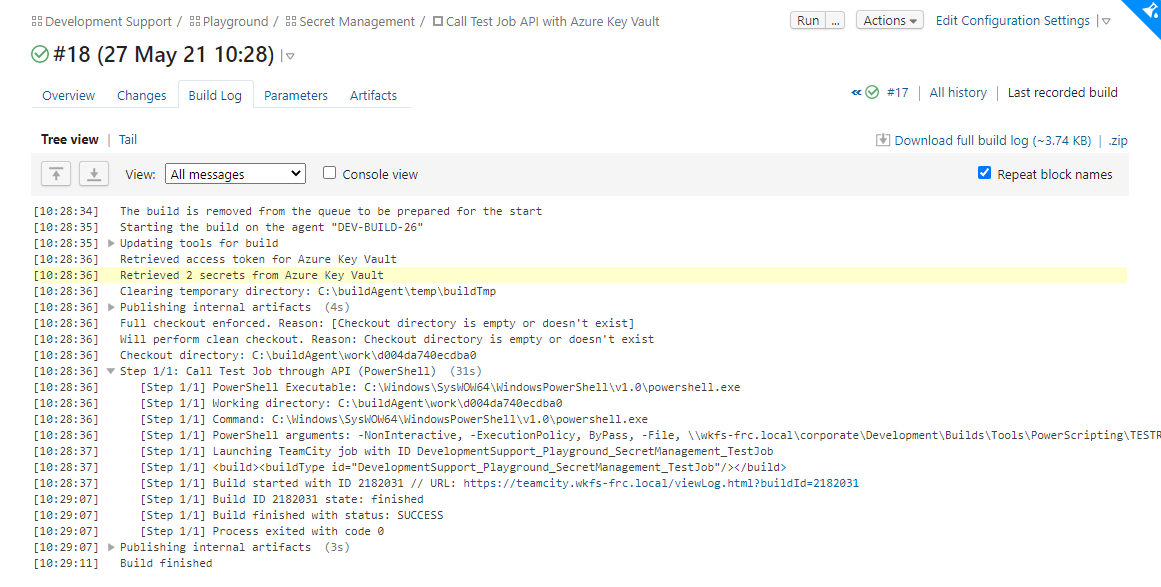
\includegraphics[width=1\textwidth]{bachproef/img/poc/script1output.png}}
    \subfigure[secrets request en printen hiervan]{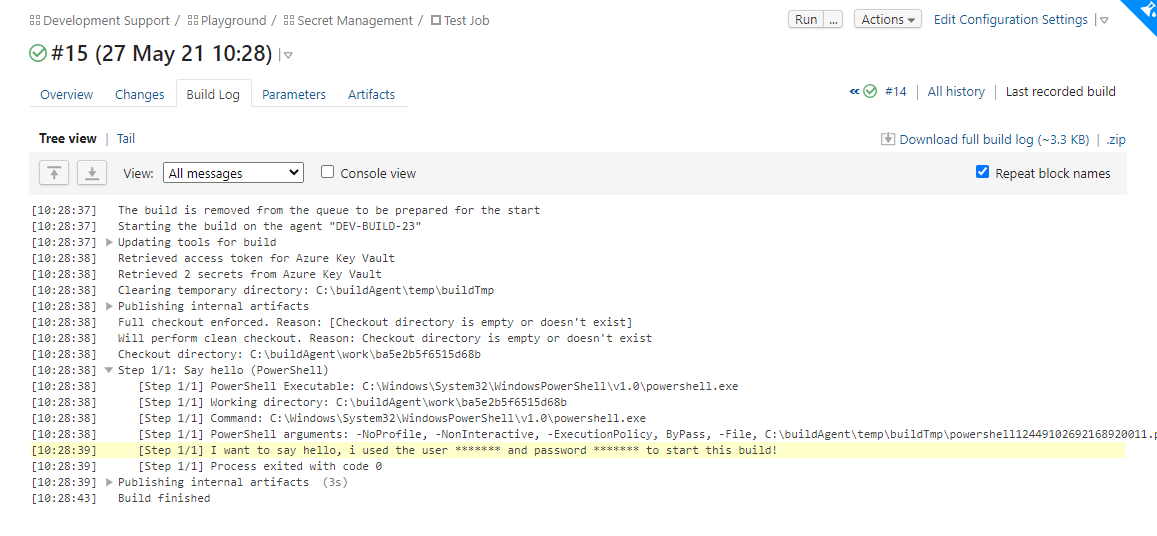
\includegraphics[width=1\textwidth]{bachproef/img/poc/script2output.png}} 
    \caption{Build logs van azure key vault werking \autocite{teamcity}}
    \label{fig:azurescripts}
\end{figure}
\newpage

Voor Hashicorp Vault is deze werking niet gelukt. De configuraties van Vault zijn juist uitgevoerd en de approle is juist ingesteld voor TeamCity waarmee de connectiviteitstest succesvol voltooid, dit wordt afgebeeld in figuur \ref{fig:approlec}. De plugin die gebruikt is faalt om de omgevingsvariabelen op te merken met de nodige gebruikte syntaxis. Waar het probleem bij ligt is niet meteen duidelijk maar het is wel duidelijk dat bij de builds geen logboekvermeldingen komen in verband met de Hashicorp Vault Plugin. Deze testen zijn gebeurt op zowel Windows als Linux agents en twee instanties van TeamCity. Als laatste wordt er in figuur \ref{fig:project} het secrets management project afgebeeld met lopende builds.

\begin{figure}[htbp]
\centerline{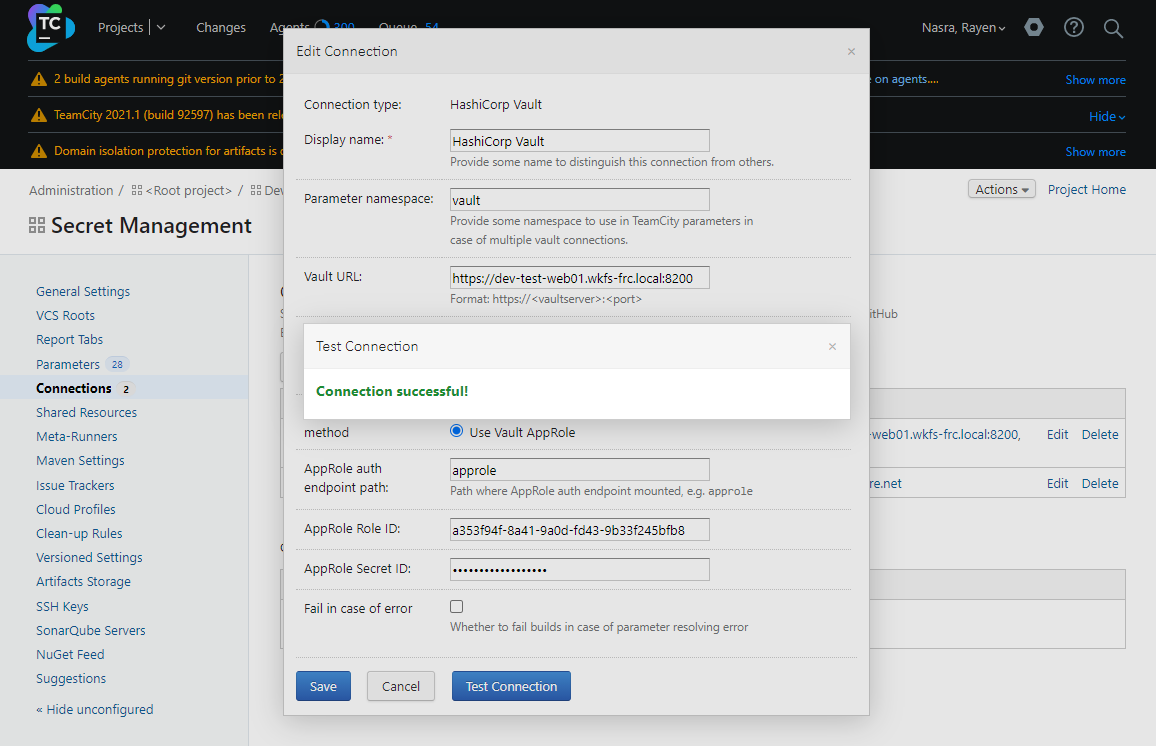
\includegraphics[width=300]{bachproef/img/poc/test connection.png}}
\caption{Connectiviteitstest TLS verbinding in WK domein, met approle TeamCity \autocite{teamcity}}
\label{fig:approlec}
\end{figure}

\begin{figure}[htbp]
\centerline{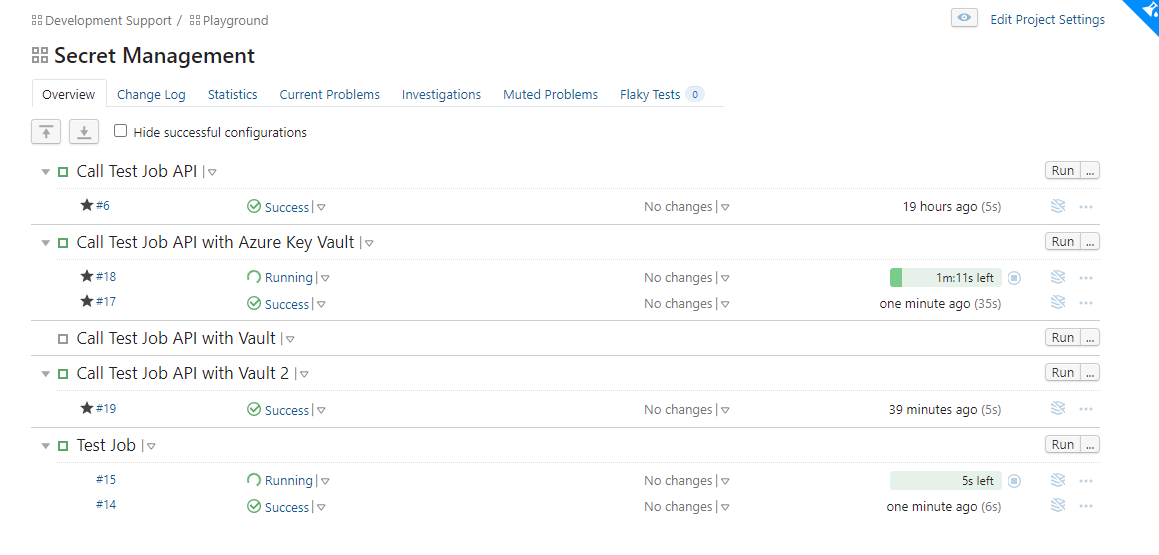
\includegraphics[width=400]{bachproef/img/poc/lopendebuilds.png}}
\caption{Secrets Management project in TeamCity met lopende builds \autocite{teamcity}}
\label{fig:project}
\end{figure}